\documentclass[10pt, twocolumn]{article}
\usepackage[utf8]{inputenc}
\usepackage{amsmath, tikz}
\usepackage{pgfplotstable}
\usepackage{graphicx}
\usepackage{subcaption}
\usepackage[margin=1in]{geometry}
\usepackage[colorlinks = true]{hyperref}

\usetikzlibrary{plotmarks}
\usetikzlibrary{calc}

\pgfdeclarelayer{bg}
\pgfsetlayers{bg, main}

\newcommand{\legendline}[1]{\parbox{1em}{{\color{#1}\rule{1em}{2pt}}}}

\newcommand{\plotsetup}[6]{
	\pgfmathsetmacro{\xleft}{#1}
	\pgfmathsetmacro{\xright}{#2}
	\pgfmathsetmacro{\ybot}{#3}
	\pgfmathsetmacro{\ytop}{#4}
	\draw[gray!25, thin, step=1cm] ({\xleft + 0.01}, {\ybot + 0.01}) grid ({\xright - 0.01}, {\ytop - 0.01});
%	\draw[gray!25, dashed, thin, step = 0.5] ({\xleft + 0.01}, {\ybot + 0.01}) grid ({\xright - 0.01}, {\ytop - 0.01});
	\draw[thick, ->] (\xleft,0) -- (\xright,0) node[pos=1, right]{#5};
	\draw[thick, ->] (0,\ybot) -- (0,\ytop) node[pos=1, above]{#6};
}

\title{Othello Experiments: 0\textsuperscript{th} Iteration\\{\small Proof of Concept}}
\author{V. Markos}
\date{\today}

\begin{document}
	\maketitle
	
	\begin{abstract}
		In this brief report we summarize any results obtained from playing Othello using various toy policies against a random agent. Throughout this report, we discuss the proposed experimental setup, possible extensions and present a plan for future iterations.
	\end{abstract}
	
	\section{Experimental Setup}
	In this series of experiments, we have used $N=3$ different policies, $p_i$, $i=1,2,3$, each being a refinement of the previous one --- all policies are shown in Figure~\ref{fig:policies01}. Using each of these, we play $M=1000$ games against a random agent, with Prudens playing always with black pieces. For each game, we keep track of the time it takes each agent to make their move as well as of the final score of the game. In this context, a game's \emph{score} is defined as the difference between white and black pieces on board. So, positive scores mean that the random agent wins, negative ones that our agent wins and zeros correspond to draws.
	
	\begin{figure}[!htb]
		\centering
		\begin{subfigure}{0.45\textwidth}
			\begin{subfigure}{\textwidth}
				\begin{verbatim}
					@Knowledge
					D1 :: legalMove(X,Y) implies
					    move(X,Y);
				\end{verbatim}\ \\[-4\topsep]
				\caption{Policy $p_1$.}
				\label{fig:policyp1}
			\end{subfigure}%
			\ \\[\topsep]
			\begin{subfigure}{\textwidth}
				\begin{verbatim}
					@KnowledgeBase
					D1 :: legalMove(X,Y) implies 
					    move(X,Y);
					D2 :: legalMove(X,Y), legalMove(Z,W),
					corner(Z,W), -?=(X,Z) implies
					    -move(X,Y);
					D3 :: legalMove(X,Y), legalMove(Z,W),
					corner(Z,W), -?=(Y,W) implies
					    -move(X,Y);
					C1 :: implies corner(0, 0);
					C2 :: implies corner(0,7);
					C3 :: implies corner(7,0);
					C4 :: implies corner(7,7);
					R1 :: legalMove(X,Y), corner(X,Y)
					implies move(X,Y);
				\end{verbatim}\ \\[-4\topsep]
				\caption{Policy $p_2$.}
				\label{fig:policyp2}
			\end{subfigure}%
		\end{subfigure}%
		\ \\[\topsep]		
		\begin{subfigure}{0.45\textwidth}
			\begin{verbatim}
				@KnowledgeBase
				D1 :: legalMove(X,Y) implies
				    move(X,Y);
				D2 :: legalMove(X,Y), legalMove(Z,W), 
				    corner(Z,W), -?=(X,Z) implies
				    -move(X,Y);
				D3 :: legalMove(X,Y), legalMove(Z,W), 
				    corner(Z,W), -?=(Y,W) implies
				    -move(X,Y);
				C1 :: implies corner(0, 0);
				C2 :: implies corner(0,7);
				C3 :: implies corner(7,0);
				C4 :: implies corner(7,7);
				R1 :: legalMove(X,Y), corner(X,Y)
				    implies move(X,Y);
				R2 :: corner(X,Y), legalMove(Z,W),
				    ?isAdj(X,Y,Z,W) implies
				    -move(Z,W);
				
				@Procedures
				function isAdj(x,y,z,w) {
				const X = parseInt(x);
				const Y = parseInt(y);
				const Z = parseInt(z);
				const W = parseInt(w);
				return Z-X < 2 && X-Z < 2 && W-Y < 2
				    && Y-W < 2 && (X != Z || Y != W);
				}
			\end{verbatim}\ \\[-4\topsep]
			\caption{Policy $p_3$.}
			\label{fig:policyp3}
		\end{subfigure}%
		\caption{All three policies used in this series of experiments.}
		\label{fig:policies01}
	\end{figure}
	
	\section{Results}
	We present some brief results in Figures~\ref{fig:results01}, \ref{fig:results02} and \ref{fig:results03}. Starting with Figure~\ref{fig:results01}, we present the average scores for all three policies used, with vertical bars denoting standard deviation. We observe there that, as expected, as policies get more refined, the performance of our agent improves significantly. Using $p_1$, which corresponds to playing at random, naturally leads to an average score close to $0$, while $p_2$, which corresponds to playing at random but for the cases where one can play on the board's corners, leads to a significantly improved performance for the black. Similarly, $p_3$, which corresponds to playing on corners when possible and, at the same time, avoid playing on cells next to corners also leads to significantly improved performance.
	
	In Figure~\ref{fig:results02} we present the absolute numbers of wins, draws and loses of all three policies. Verifying results shown in Figure~\ref{fig:results01}, we observe that as the underlying policy becomes more sophisticated, the performance of our agent also improves. In Figure~\ref{fig:results02}, this is reflected mostly on the numbers of wins and loses (blue and red curves, respectively), while the number of draws remains virtually constant.
	
	Finally, Figure~\ref{fig:results03} demonstrates again the positive correlation between policy sophistication and performance, using score distributions. As demonstrated there, while score distribution for $p_1$ is relatively symmetric\footnote{Actually, slightly skewed towards positive scores, i.e., loses.}, introducing more elaborate heuristics to our agent's policy significantly skews the score distribution towards negative values, i.e., wins for our agent.
	
	\begin{figure}[!htb]
		\centering
		\begin{tikzpicture}[x = 1cm, y = 0.1cm]
			\plotsetup{-0.1}{4}{-35}{21}{Policies}{Avg score}
			\foreach \i in {20, 10, ..., -30} {
				\node[left, xshift=-0.5mm, anchor=east] (y\i) at (0,\i) {\small$\i$};
			}
			\draw[red, thick, xshift=1cm] plot[mark=square*] file {../plots/avgScores/allPolicies.table};
			% STDs
			\pgfplotstableread{../plots/avgScores/stds.table}\table
			\pgfplotstablegetrowsof{\table}
			\pgfmathsetmacro{\ROWS}{\pgfplotsretval-1}
			\pgfplotstablegetcolsof{\table}
			\pgfmathsetmacro{\COLS}{\pgfplotsretval-1}
			%
			\foreach \row in {0,...,\ROWS} {
				\foreach \col in {0,...,\COLS} {
					\pgfplotstablegetelem{\row}{[index]\col}\of\table
					\ifnum\col=0
						\xdef\x{\pgfplotsretval}
					\fi
					\ifnum\col=1
						\xdef\avg{\pgfplotsretval}
					\fi
					\ifnum\col=2
						\xdef\std{\pgfplotsretval}
					\fi
				}
				\draw[red, thin, |-|, xshift = 1cm] (\x,{\avg - \std}) -- (\x,{\avg + \std});
			}
		\end{tikzpicture}
		\caption{Average score for each policy, $p_1,p_2,p_3$ (left-to-right). Vertical bars indicate standard deviation.}
		\label{fig:results01}
	\end{figure}

	\begin{figure}[!htb]
		\centering
		\begin{tikzpicture}[x = 1cm, y = 0.005cm]
		\plotsetup{-0.1}{4}{-20}{1050}{Policies}{\# of games}
		\foreach \i in {1000, 800, ..., 0} {
			\node[left, xshift=-0.5mm, anchor=east] (y\i) at (0,\i) {\small$\i$};
		}
		% STDs
		\pgfplotstableread{../plots/avgScores/scoreCounts.table}\table
		\pgfplotstablegetrowsof{\table}
		\pgfmathsetmacro{\ROWS}{\pgfplotsretval-1}
		\pgfplotstablegetcolsof{\table}
		\pgfmathsetmacro{\COLS}{\pgfplotsretval-1}
		%
		\foreach \row in {0,...,\ROWS} {
			\ifnum\row=0
				\foreach \col in {0,...,\COLS} {
					\pgfplotstablegetelem{\row}{[index]\col}\of\table
					\ifnum\col=0
						\xdef\x{\pgfplotsretval}
					\fi
					\ifnum\col=1
						\xdef\wins{\pgfplotsretval}
%					\draw[thick, blue, xshift = 1cm, mark=o] plot coordinates {(\x-1,\ywins) (\x,\wins)};
						\xdef\ywins{\wins}
					\fi
					\ifnum\col=2
						\xdef\draws{\pgfplotsretval}
%					\draw[thick, green!60!black, xshift = 1cm, mark=o] plot coordinates {(\x-1,\ydraws) (\x,\draws)};
						\xdef\ydraws{\draws}
					\fi
					\ifnum\col=3
						\xdef\loses{\pgfplotsretval}
%					\draw[thick, red, xshift = 1cm, mark=o] plot coordinates {(\x-1,\yloses) (\x,\loses)};
						\xdef\yloses{\loses}
					\fi
				}
			\else
				\foreach \col in {0,...,\COLS} {
					\pgfplotstablegetelem{\row}{[index]\col}\of\table
					\ifnum\col=0
						\xdef\x{\pgfplotsretval}
					\fi
					\ifnum\col=1
						\xdef\wins{\pgfplotsretval}
						\draw[thick, blue, xshift = 1cm, mark=o] plot coordinates {(\x-1,\ywins) (\x,\wins)};
						\xdef\ywins{\wins}
						
					\fi
					\ifnum\col=2
						\xdef\draws{\pgfplotsretval}
						\draw[thick, green!60!black, xshift = 1cm, mark=o] plot coordinates {(\x-1,\ydraws) (\x,\draws)};
						\xdef\ydraws{\draws}
					\fi
					\ifnum\col=3
						\xdef\loses{\pgfplotsretval}
						\draw[thick, red, xshift = 1cm, mark=o] plot coordinates {(\x-1,\yloses) (\x,\loses)};
						\xdef\yloses{\loses}
					\fi
				}
			\fi
		}
		\end{tikzpicture}
		\caption{Total number of wins (\legendline{blue}), draws (\legendline{green!60!black}) and loses (\legendline{red}) with respect to each policy.}
		\label{fig:results02}
	\end{figure}

	\begin{figure}[!htb]
		\centering\resizebox{\linewidth}{!}{
		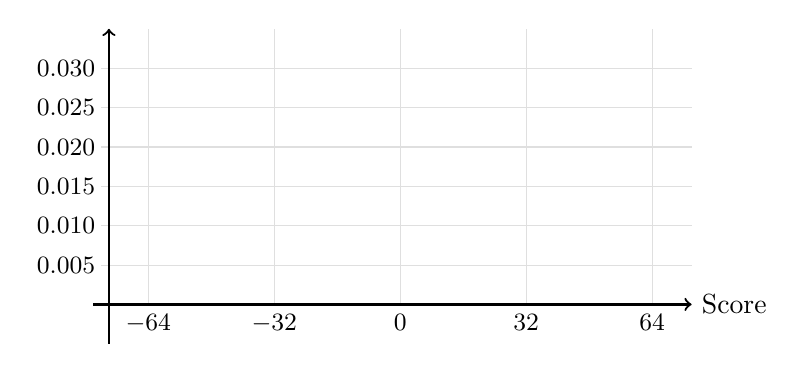
\begin{tikzpicture}[x = 0.2cm, y = 100cm]
		\draw[thick, ->] (-4,0) -- (34,0) node[pos=1, right]{Score};
		\draw[thick, ->] (-3,-0.005) -- (-3,0.035);
		\begin{pgfonlayer}{bg}
			\foreach \i in {0.030, 0.025, ..., 0.001} {
				\pgfmathsetmacro{\p}{int((int(1000 * \i) + 1))}
				\ifnum\p<10
					\node[left, xshift=-0.5mm, anchor=east] (y\i) at (-3,\i) {\small$0.00\p$};
				\else
					\node[left, xshift=-0.5mm, anchor=east] (y\i) at (-3,\i) {\small$0.0\p$};
				\fi
				\draw[gray!25, thin, shorten <= -1mm] (-3,\i) -- (34,\i);
			}
			\foreach \i in {0,8,...,32} {
				\pgfmathsetmacro{\xtick}{int(4*\i-64)}
				\node[below, anchor=north] (x\i) at ({\i-0.5},0) {\small$\xtick$};
				\draw[gray!25, thin, shorten <= -0.1mm] ({\i-0.5},0) -- ({\i-0.5},0.035);
			}
		\end{pgfonlayer}
		\draw[red, thick] plot[smooth] file {../plots/avgScores/scoreDist0.table};
		\draw[green!60!black, thick] plot[smooth] file {../plots/avgScores/scoreDist1.table};
		\draw[blue, thick] plot[smooth] file {../plots/avgScores/scoreDist2.table};
		\end{tikzpicture}}
		\caption{Score distribution per policy. $p_1$: (\legendline{red}), $p_2$: (\legendline{green!60!black}), $p_3$: (\legendline{blue}).}
		\label{fig:results03}
	\end{figure}
	
	\section{Discussion and Future Iterations}
	Given that any policies related to Othello are/will be first-order, it might be a good chance to gather some data about Prudens's performance in larger/more complex and realistic settings. Moreover, future iterations might include:
	\begin{itemize}
		\item More sophisticated policies compared to $p_3$;
		\item More ``tough'' opponents such as a \texttt{minimax} agent(utilizing $\alpha-\beta$ prunning, for instance) or (D)NNs;
		\item Replace the purely symbolic agent used in this set of experiments with a Neural-Symbolic one --- as discussed earlier on this week with Marios.
	\end{itemize}
	Lastly, we could also consider what other quantities (other than score and win/lose ratio) would make sense to plot and present, so as to sharpen our understanding of any results.
\end{document}